\scanpage{27}
$S=k\{T\}$ (polynômes à p.d.) anneau gradué à degrés $\geq0$,
$M$ un $k$-module, $N\geq0$, d'où $M\otimes_kS$ et par suite
\diagram{\begin{tikzcd}
M\otimes_kS \arrow[r] & \unsure{\varphi_N|\rho_N}\tau_N(M\otimes_kS)
\end{tikzcd}}
\uline{Thm} L'hom précédent est un isom en degrés $\geq0$, i.e. on a
\diagram{\begin{tikzcd}
(\alpha)\qquad M\otimes_kS \arrow[r,"\sim"] & \unsure{\varphi_{0N}|\rho_{0N}}\tau_N(M\otimes_kS)
\end{tikzcd}}
Enoncé équivalent:
\[
M\otimes_kS\in\operatorname{Im\,ess}\varphi_{0N}\qquad(\forall N\geq0)
\]
ou encore
\[
M\otimes_kS\in\operatorname{Im\,ess}\varphi_{0,\infty}
\]

\uline{NB} En degrés $\geq N$, c'est clair que $\alpha$ est un isom, il suffit donc de regarder les degrés $0\leq i<N$. Le cas $i=0$ a été traité déjà par une démonstration spéciale (\unsure{on la retrouvera} dans \unsure{la dém. qui va suivre}).

Reformulation du \uline{Thm}

Si $0\leq i\leq N$, \unsure{on a}
\diagram{\begin{tikzcd}
\left(\begin{array}{c}\xi T^{(i)}\\\uparrow\\\xi\end{array}\right) & (M\otimes_k\unsure{S})_i \arrow[r,"\sim"] & \operatorname{Hom}^{i}(\tau_{N-i}(S),M\otimes_kS)\\
& M \arrow[u,phantom,"\wr" description] &
\end{tikzcd}}
(seul le cas $0\leq i<N$ doit être établi)

\uline{Cor}
\[
\operatorname{Ext}^n(\tau_{N-i}(S)[-i],M\otimes_kS)=0\quad\text{si }n>0
\]
$\forall i\geq0$ (seul le cas $i<N$ est non trivial \deleted{$\unsure{0\leq i}$})

Ce théorème équivaut à l'énoncé suivant, où $k$ ne figure plus

\uline{Th} Soient $0\leq i\leq N$ deux entiers, $M$ un $\mathbf Z$-module, $(\xi_k)_{k\geq N}$ une famille d'éléments de $M$, telle que l'on ait
\figure{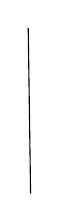
\begin{tikzpicture}\draw (0,0) -- (0.03,-2.1);\end{tikzpicture}}
\[
(1)\qquad c_{\ell,k}\xi_k=c_{\ell,k-i}\xi_{k+\ell}\qquad\text{pour }k\geq N,\ \ell\geq0
\]
\mspage{26}
